\documentclass{standalone}
\usepackage{tikz}

\input{definitions.tex}
../../ndlfilters/notation_def.tex
\input{graphicalModels.tex}
% Requires \usepackage{adjustbox}
% trim in includegraphics is left bottom right top (not easy to remember!)
\global\long\def\ricardoPicture#1{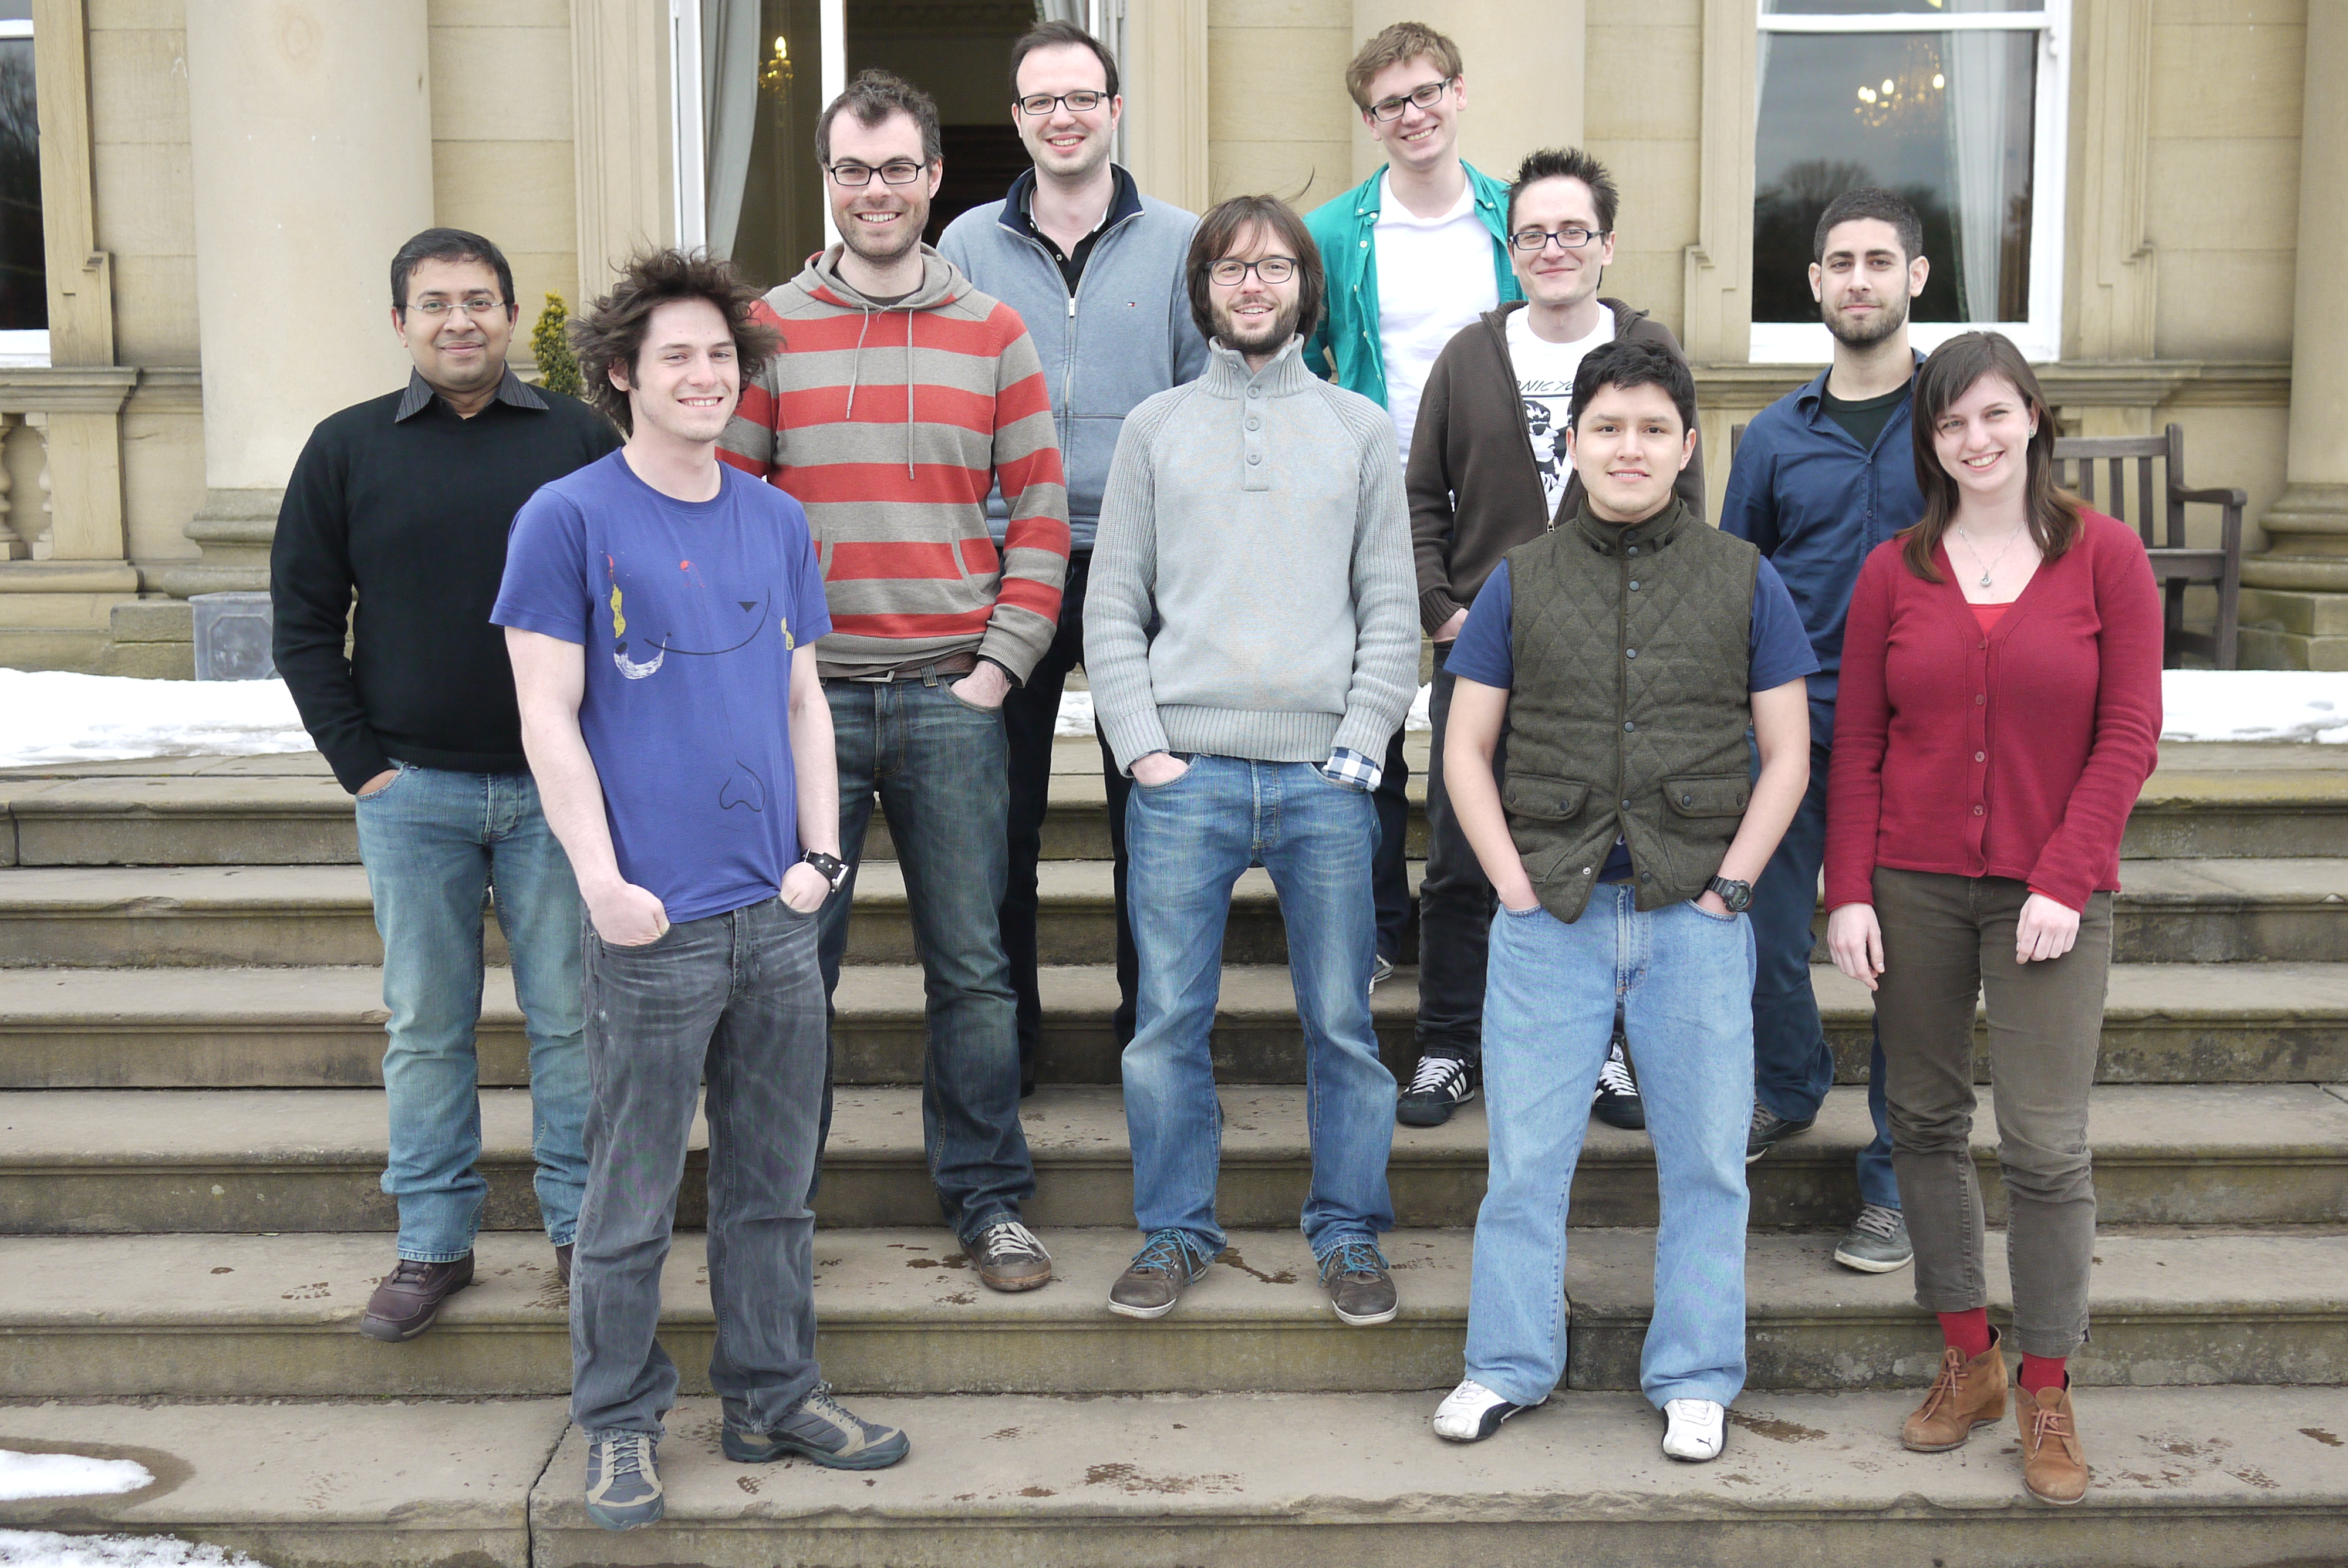
\includegraphics[trim=2662px 1780px 1110px 600px, clip,width=#1]{../../../photos/group/2013_03_28_180606.JPG}}
\global\long\def\nicoloPicture#1{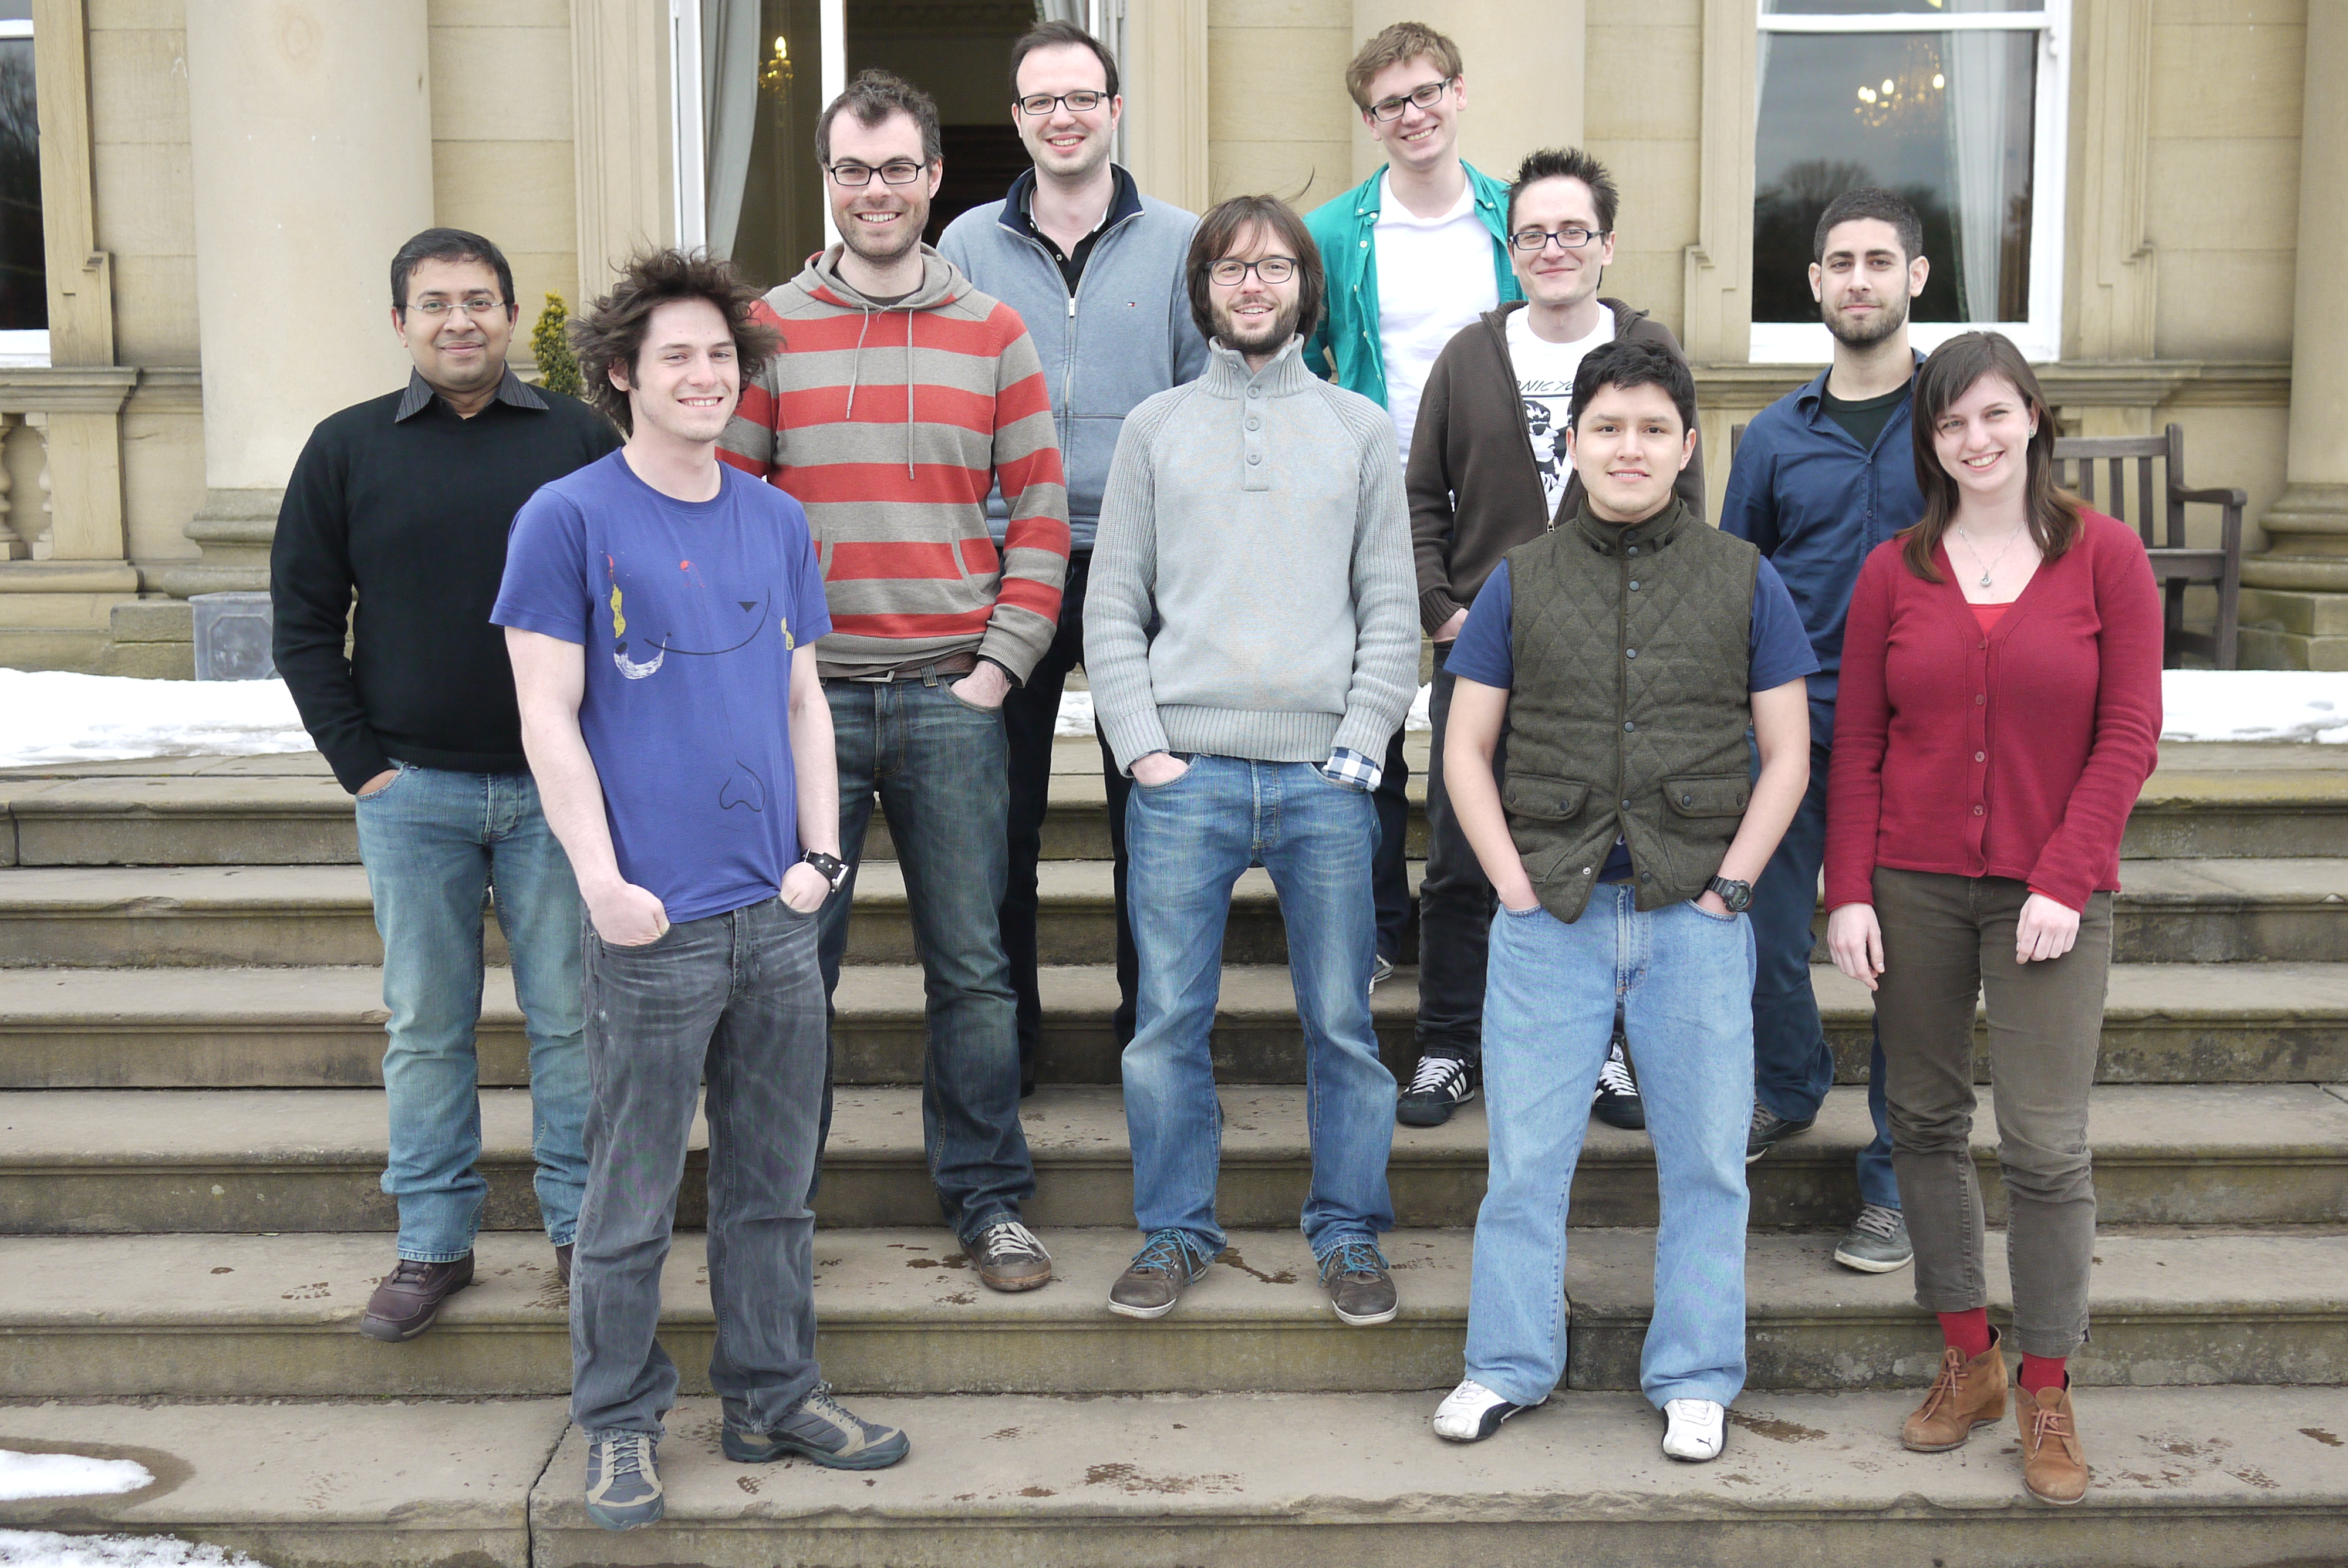
\includegraphics[trim=1718px 2360px 2090px 50px, clip,width=#1]{../../../photos/group/2013_03_28_180606.JPG}}
\global\long\def\alanPicture#1{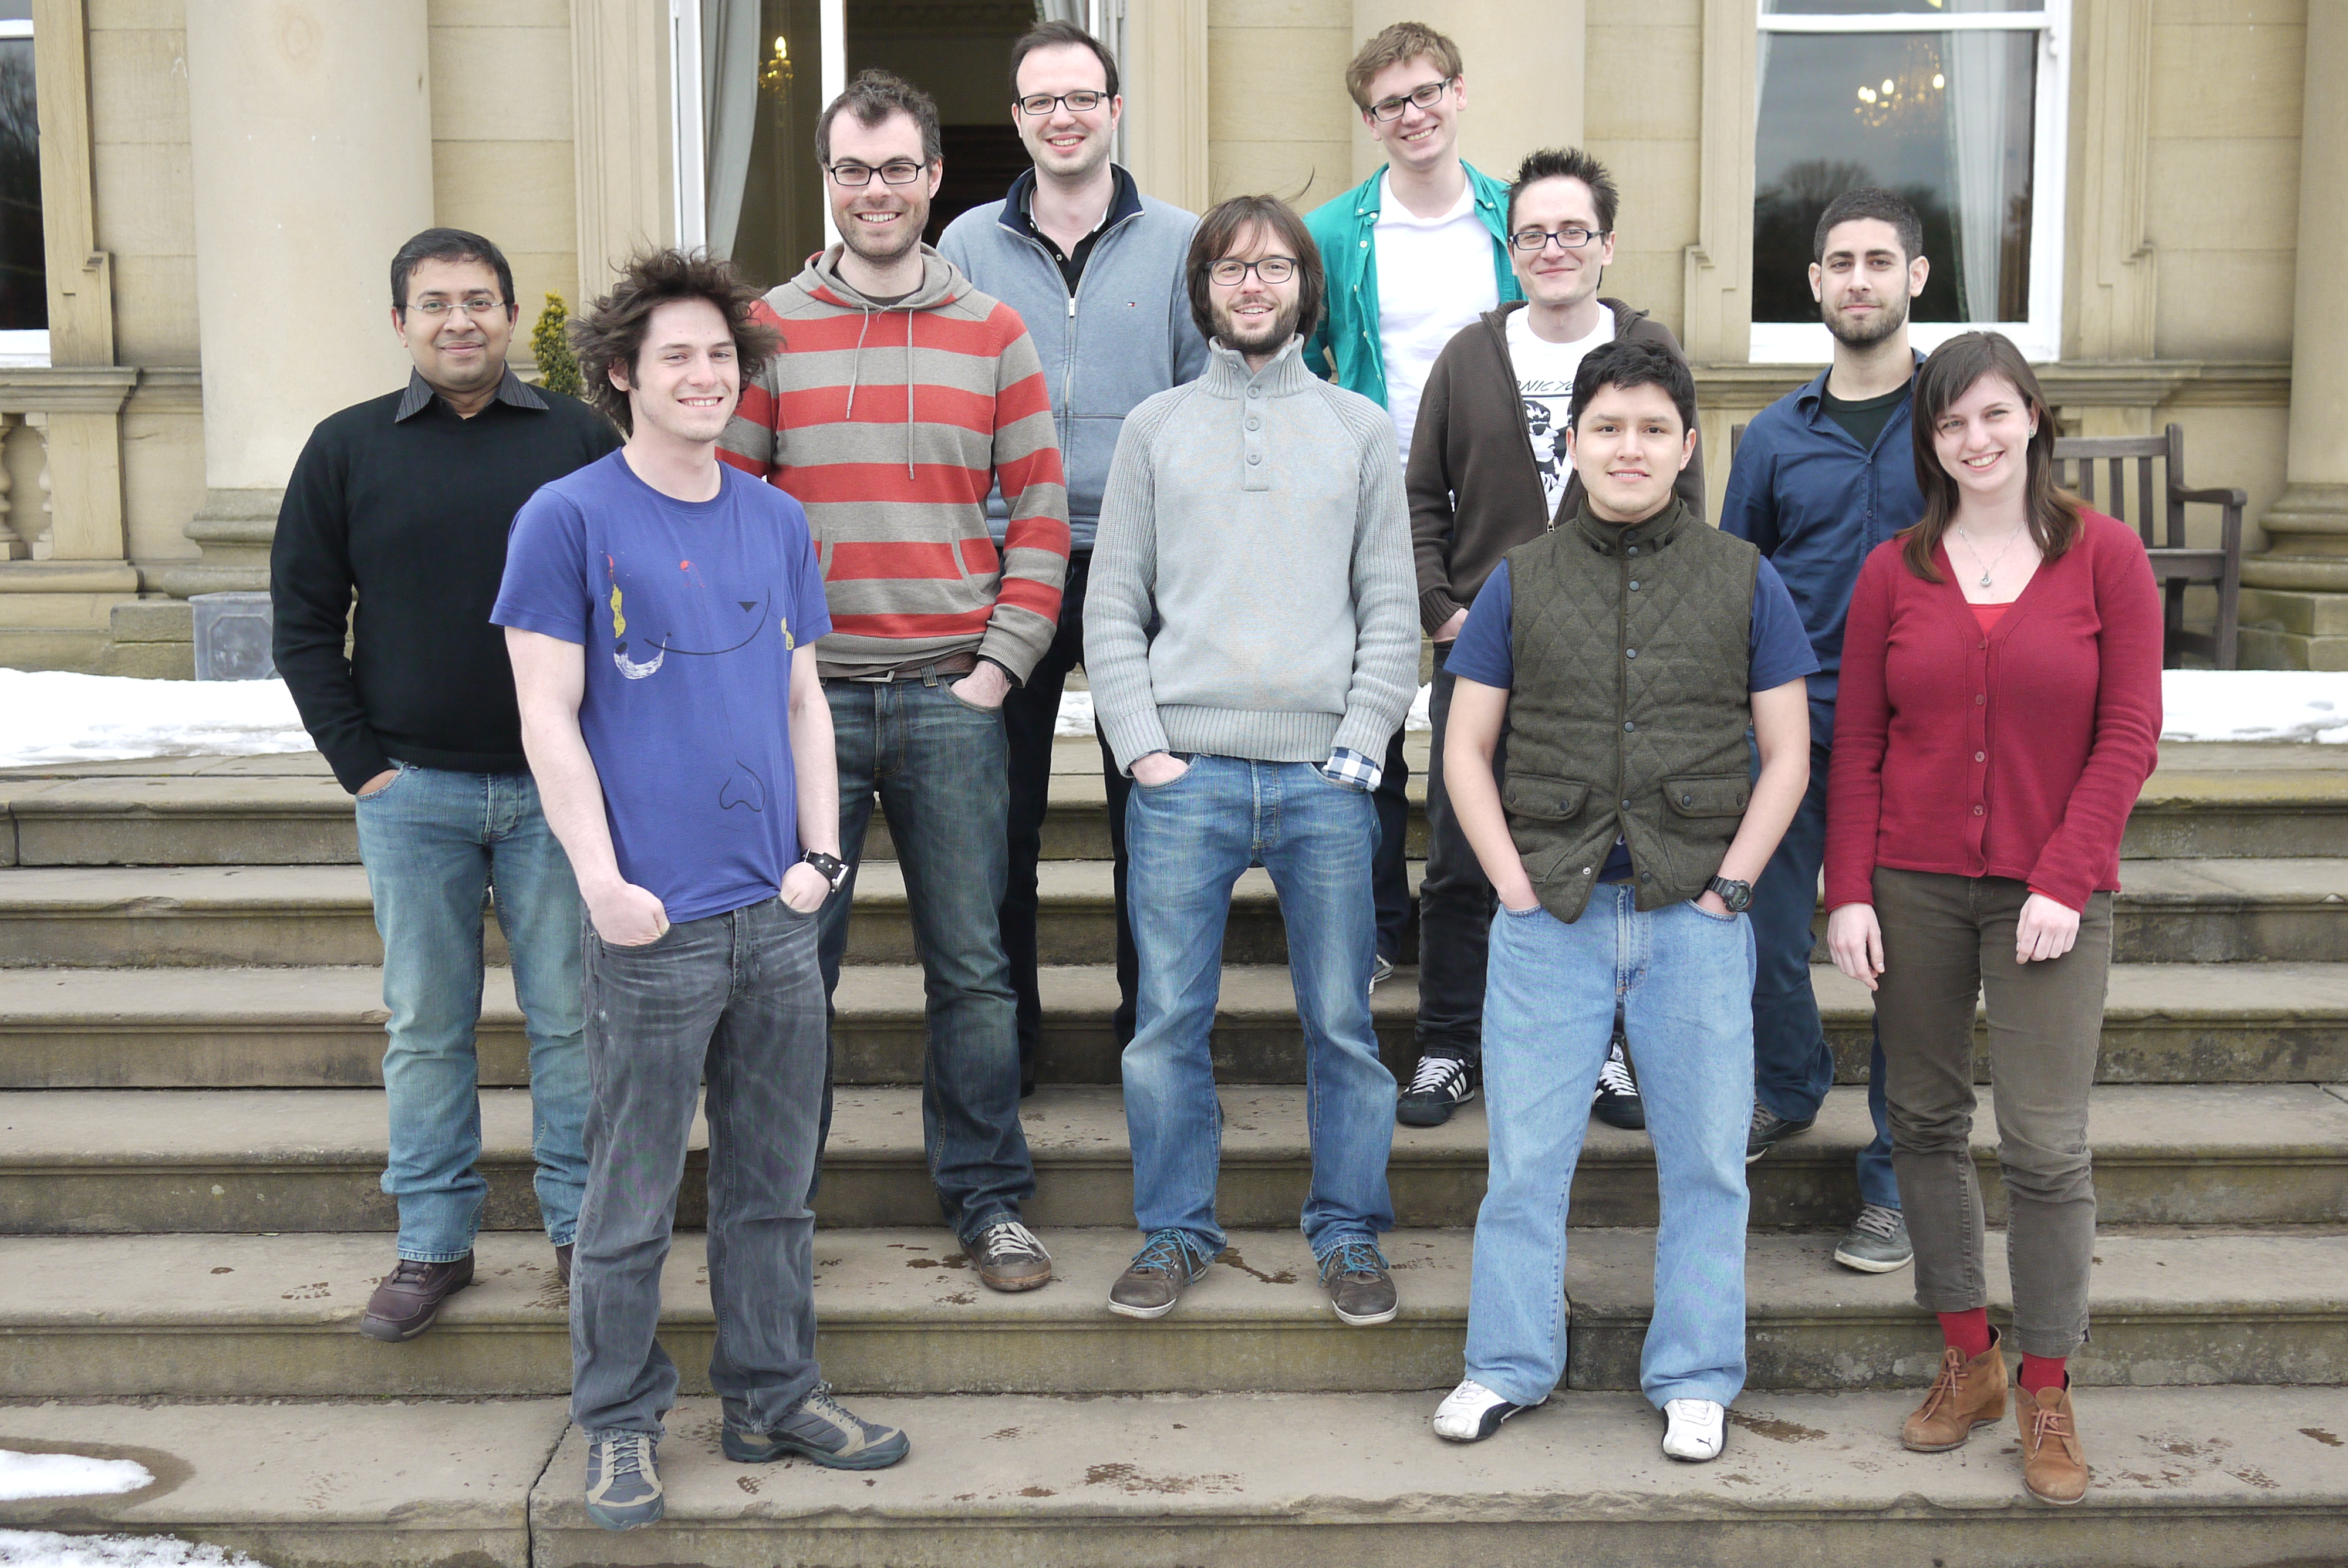
\includegraphics[trim=1076px 1920px 2730px 480px, clip,width=#1]{../../../photos/group/2013_03_28_180606.JPG}}
\global\long\def\andreasPicture#1{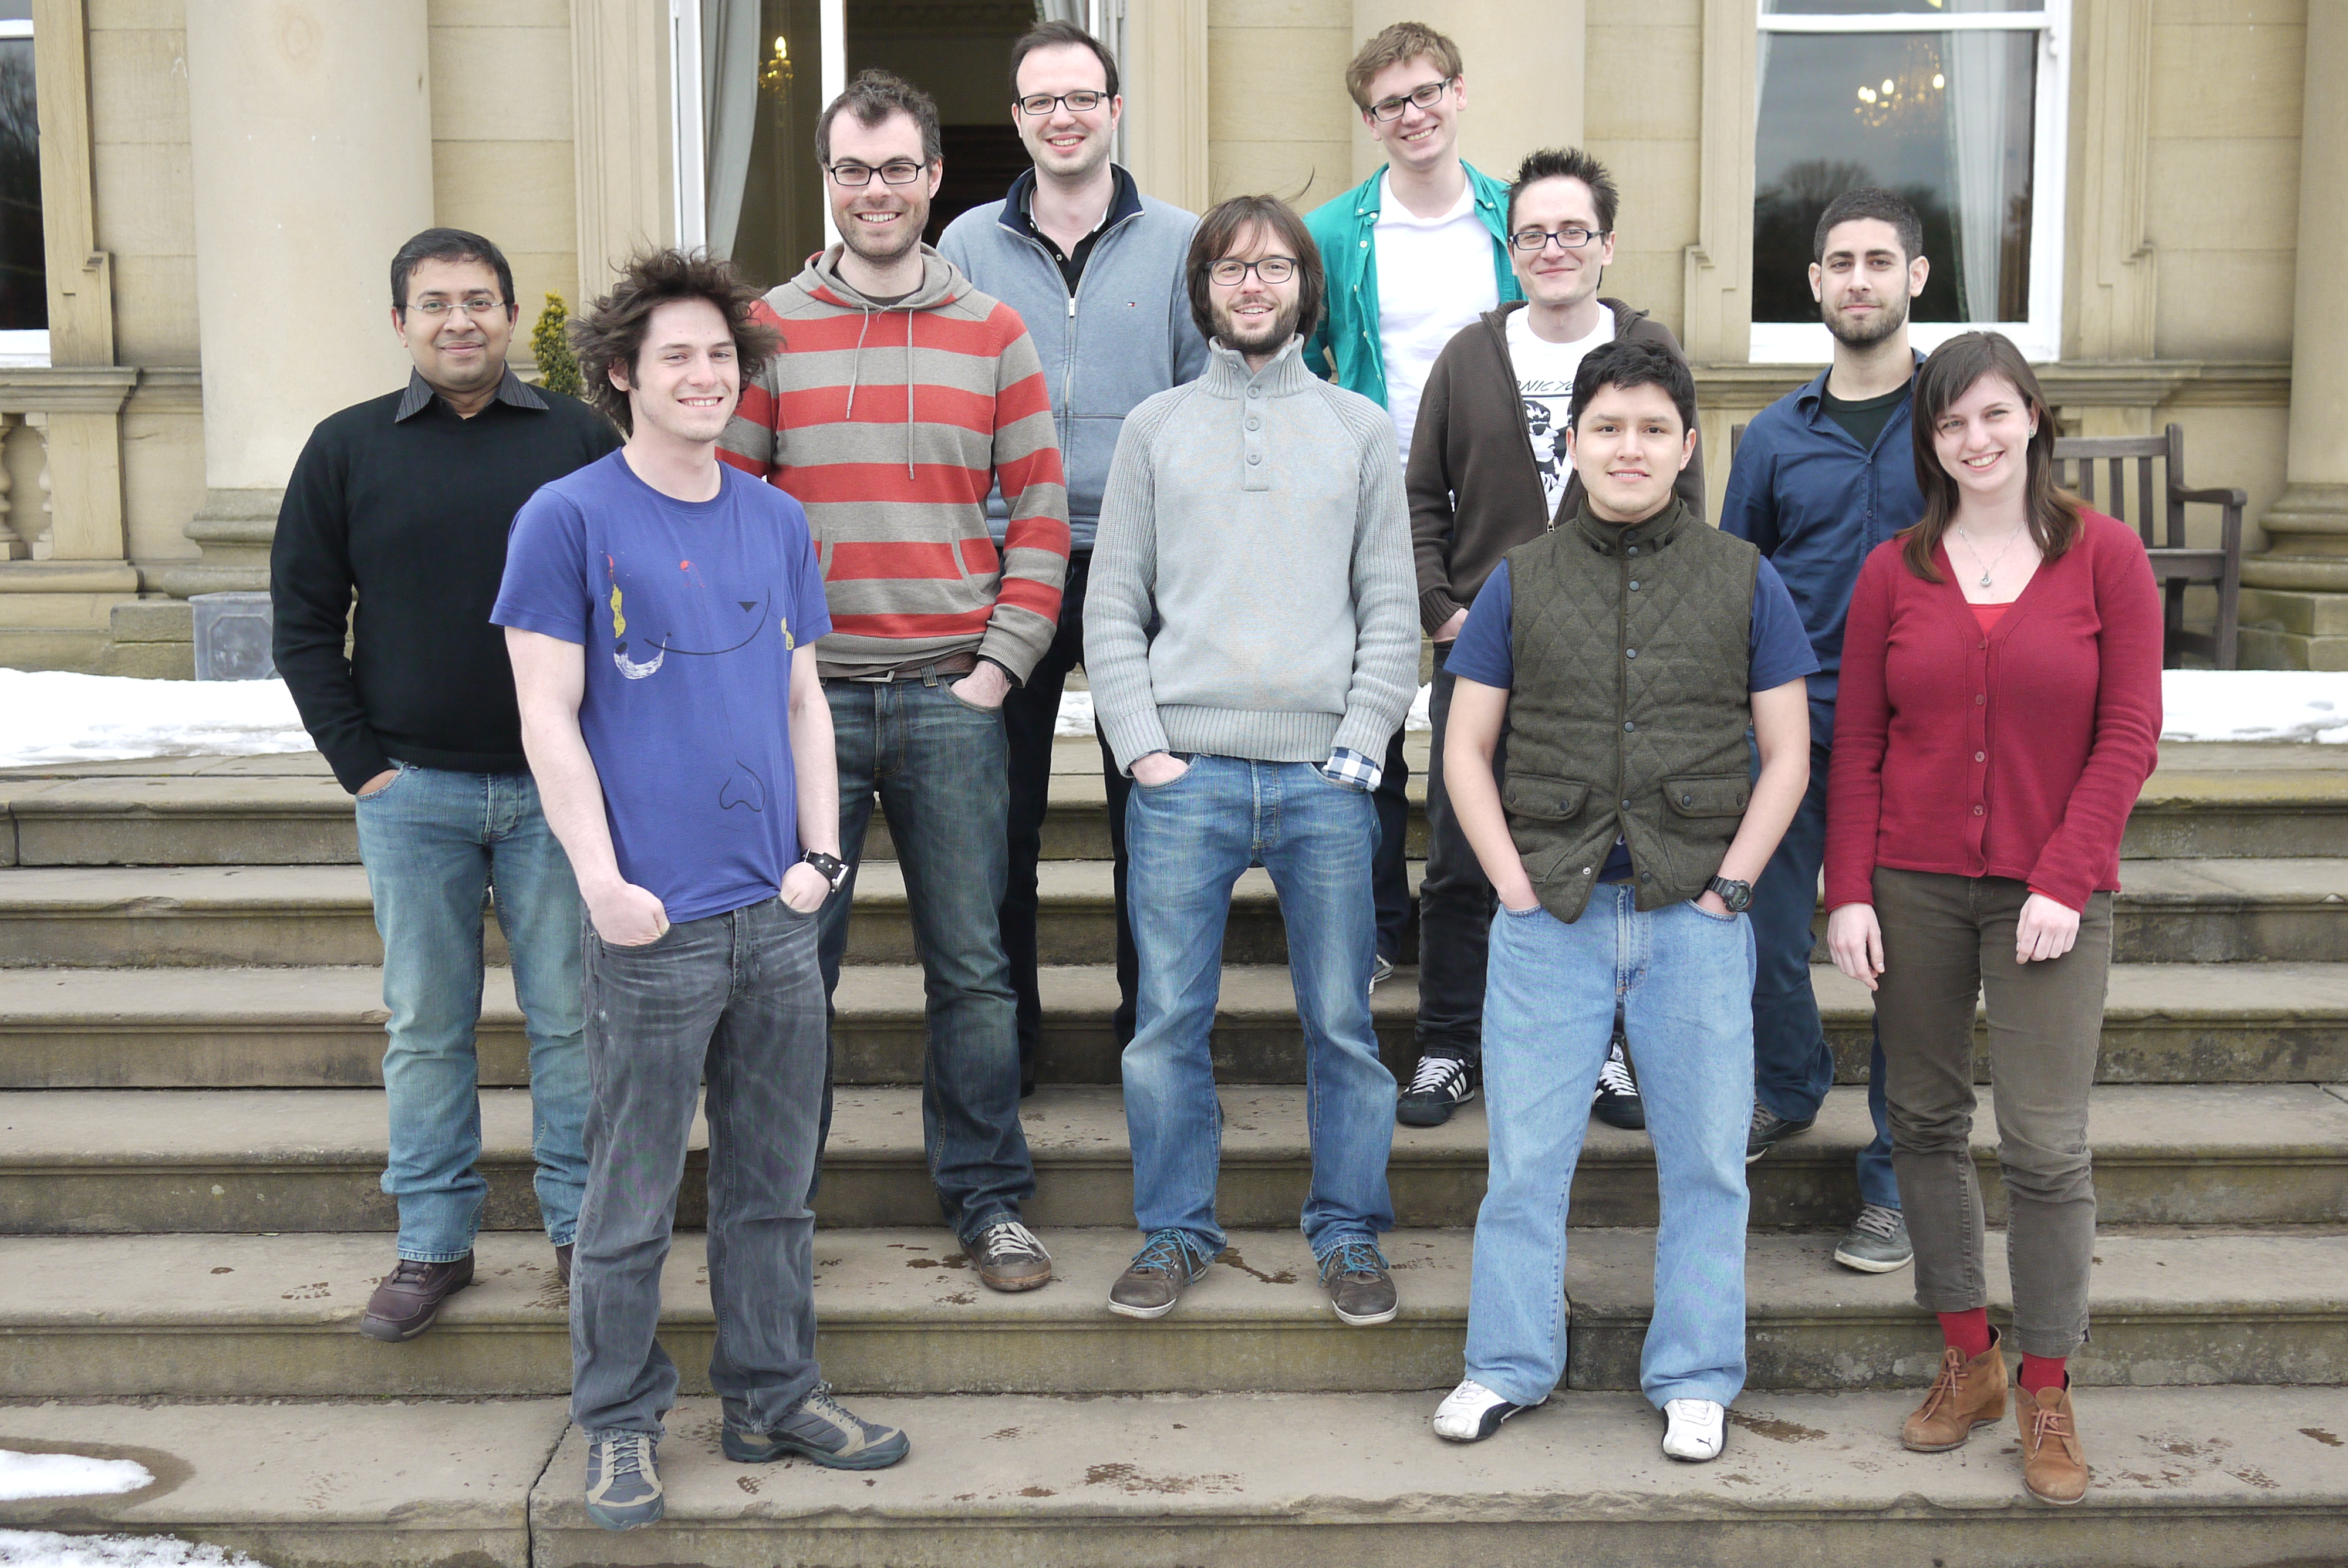
\includegraphics[trim=3090px 2080px 730px 330px, clip,width=#1]{../../../photos/group/2013_03_28_180606.JPG}}
\global\long\def\nicolasThinkingPicture#1{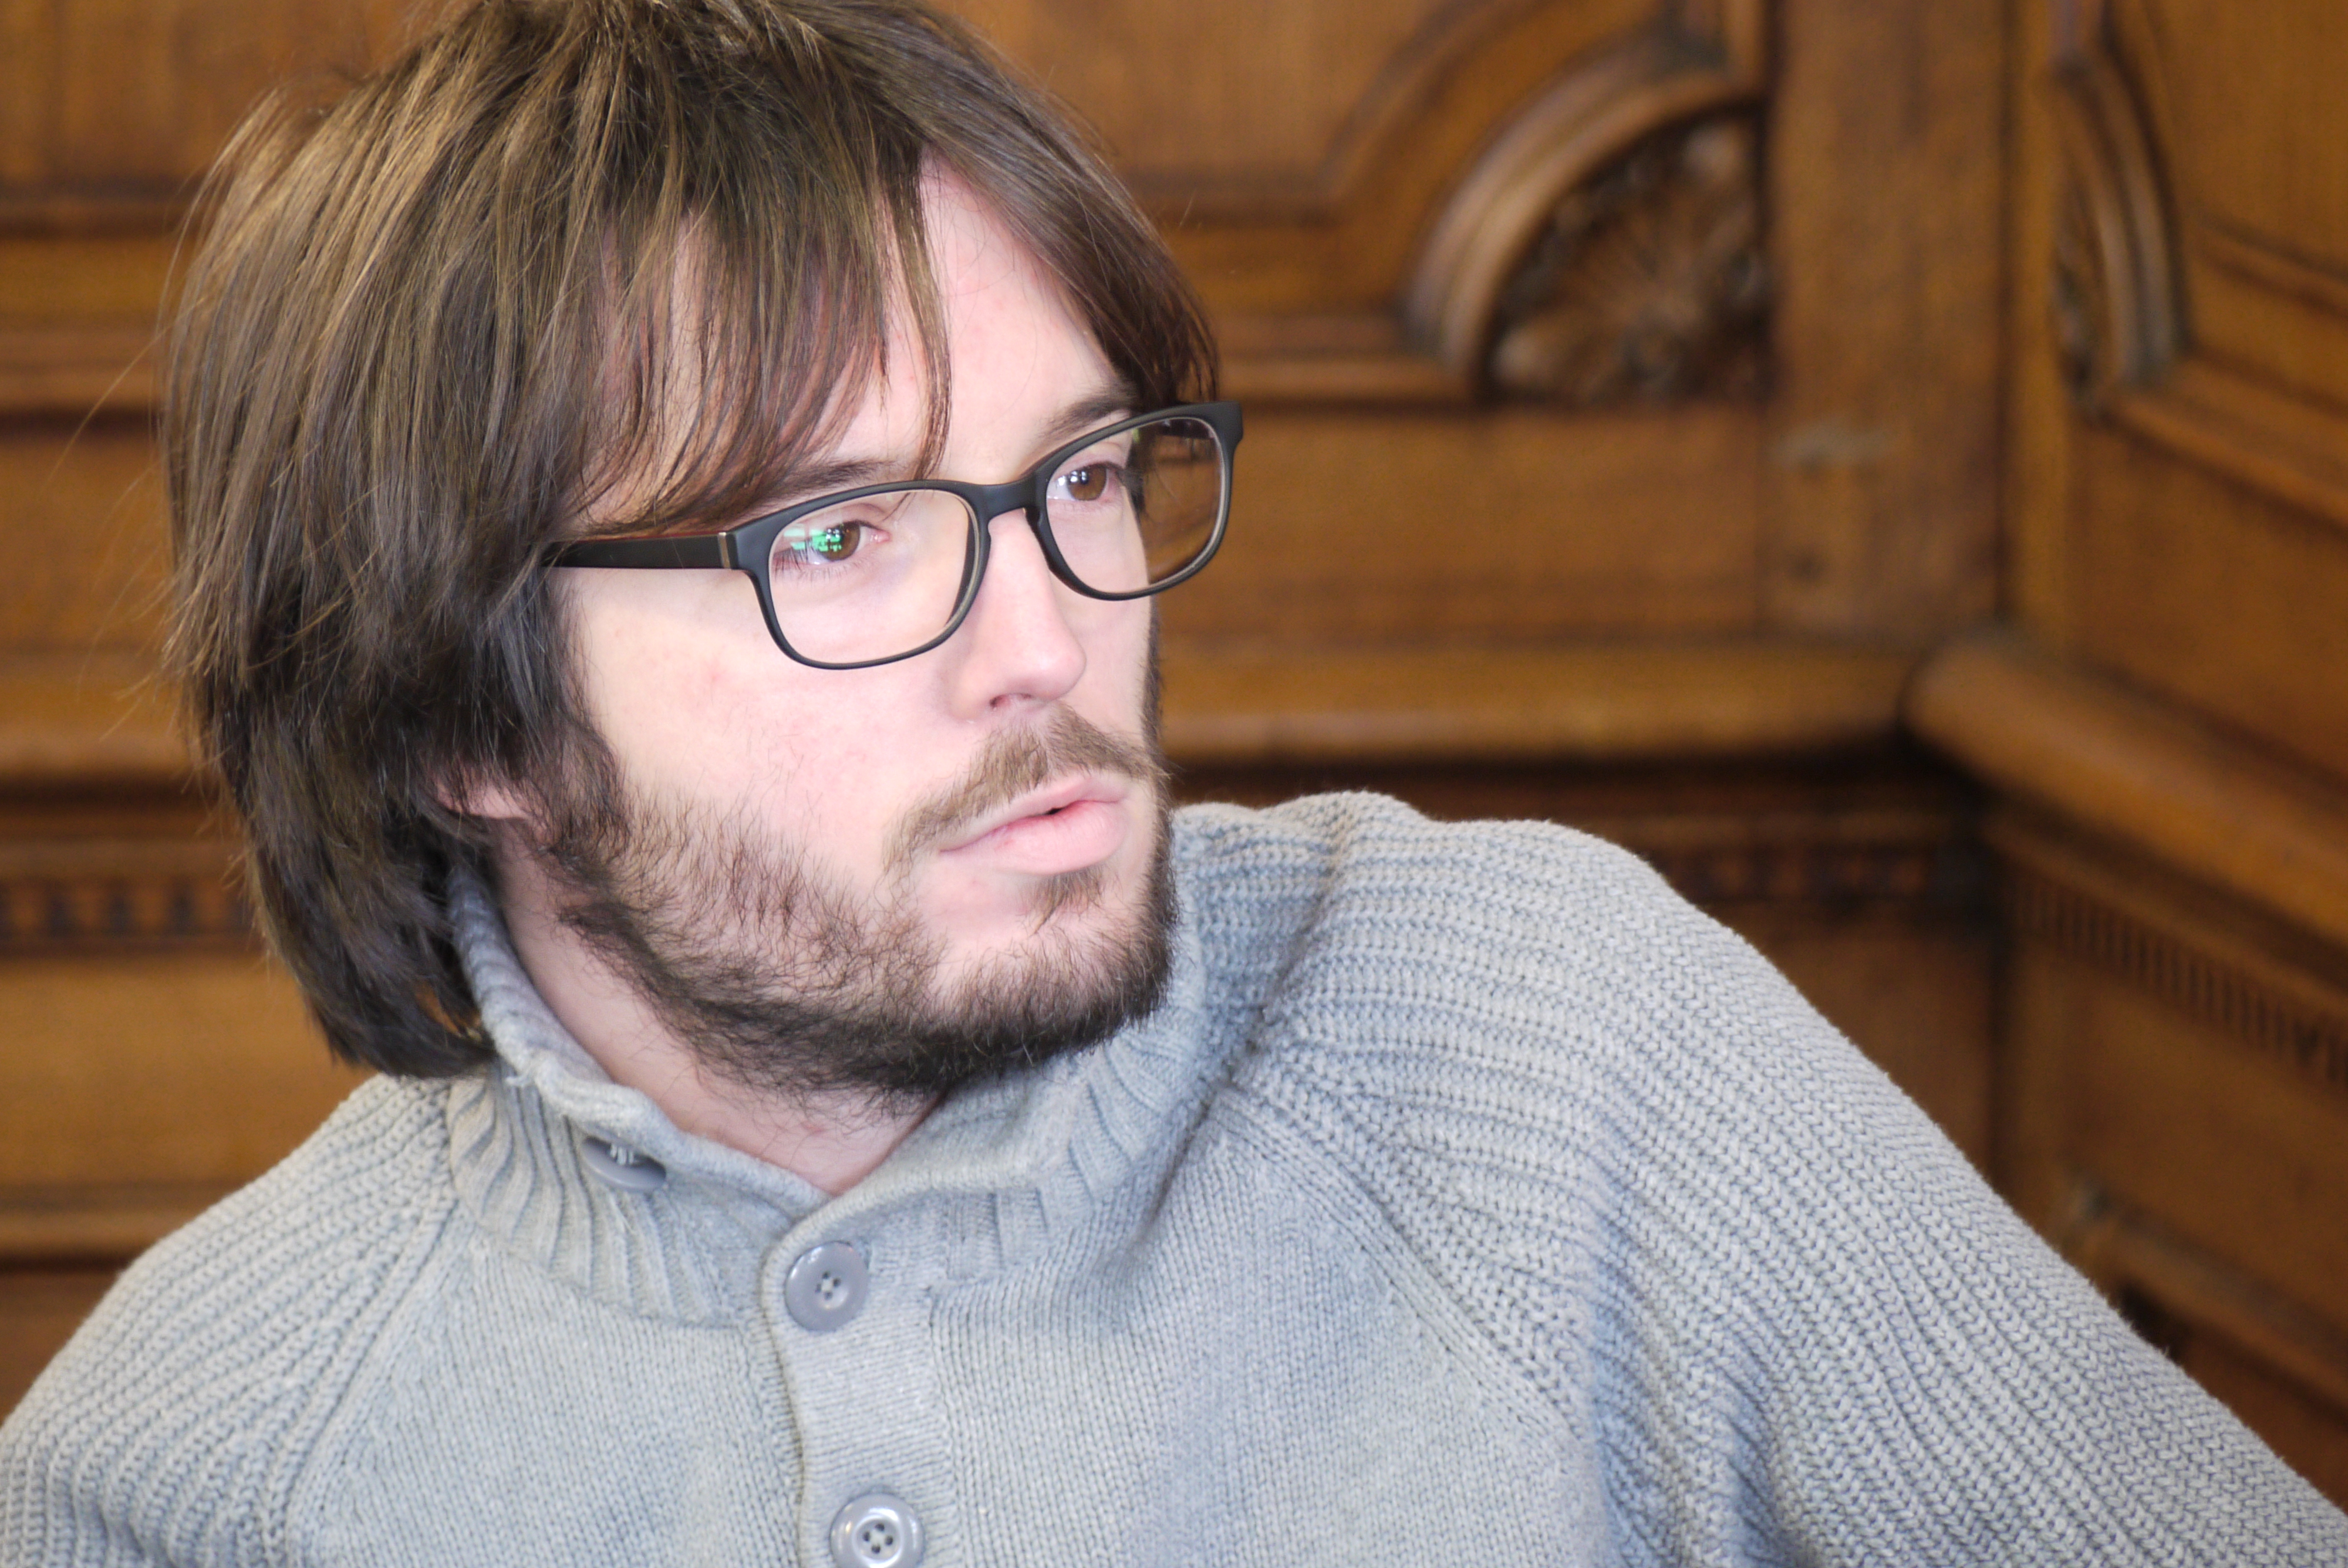
\includegraphics[trim=300px 700px 1900px 200px, clip,width=#1]{../../../photos/group/2013_03_28_114601.JPG}}
\global\long\def\jamesPicture#1{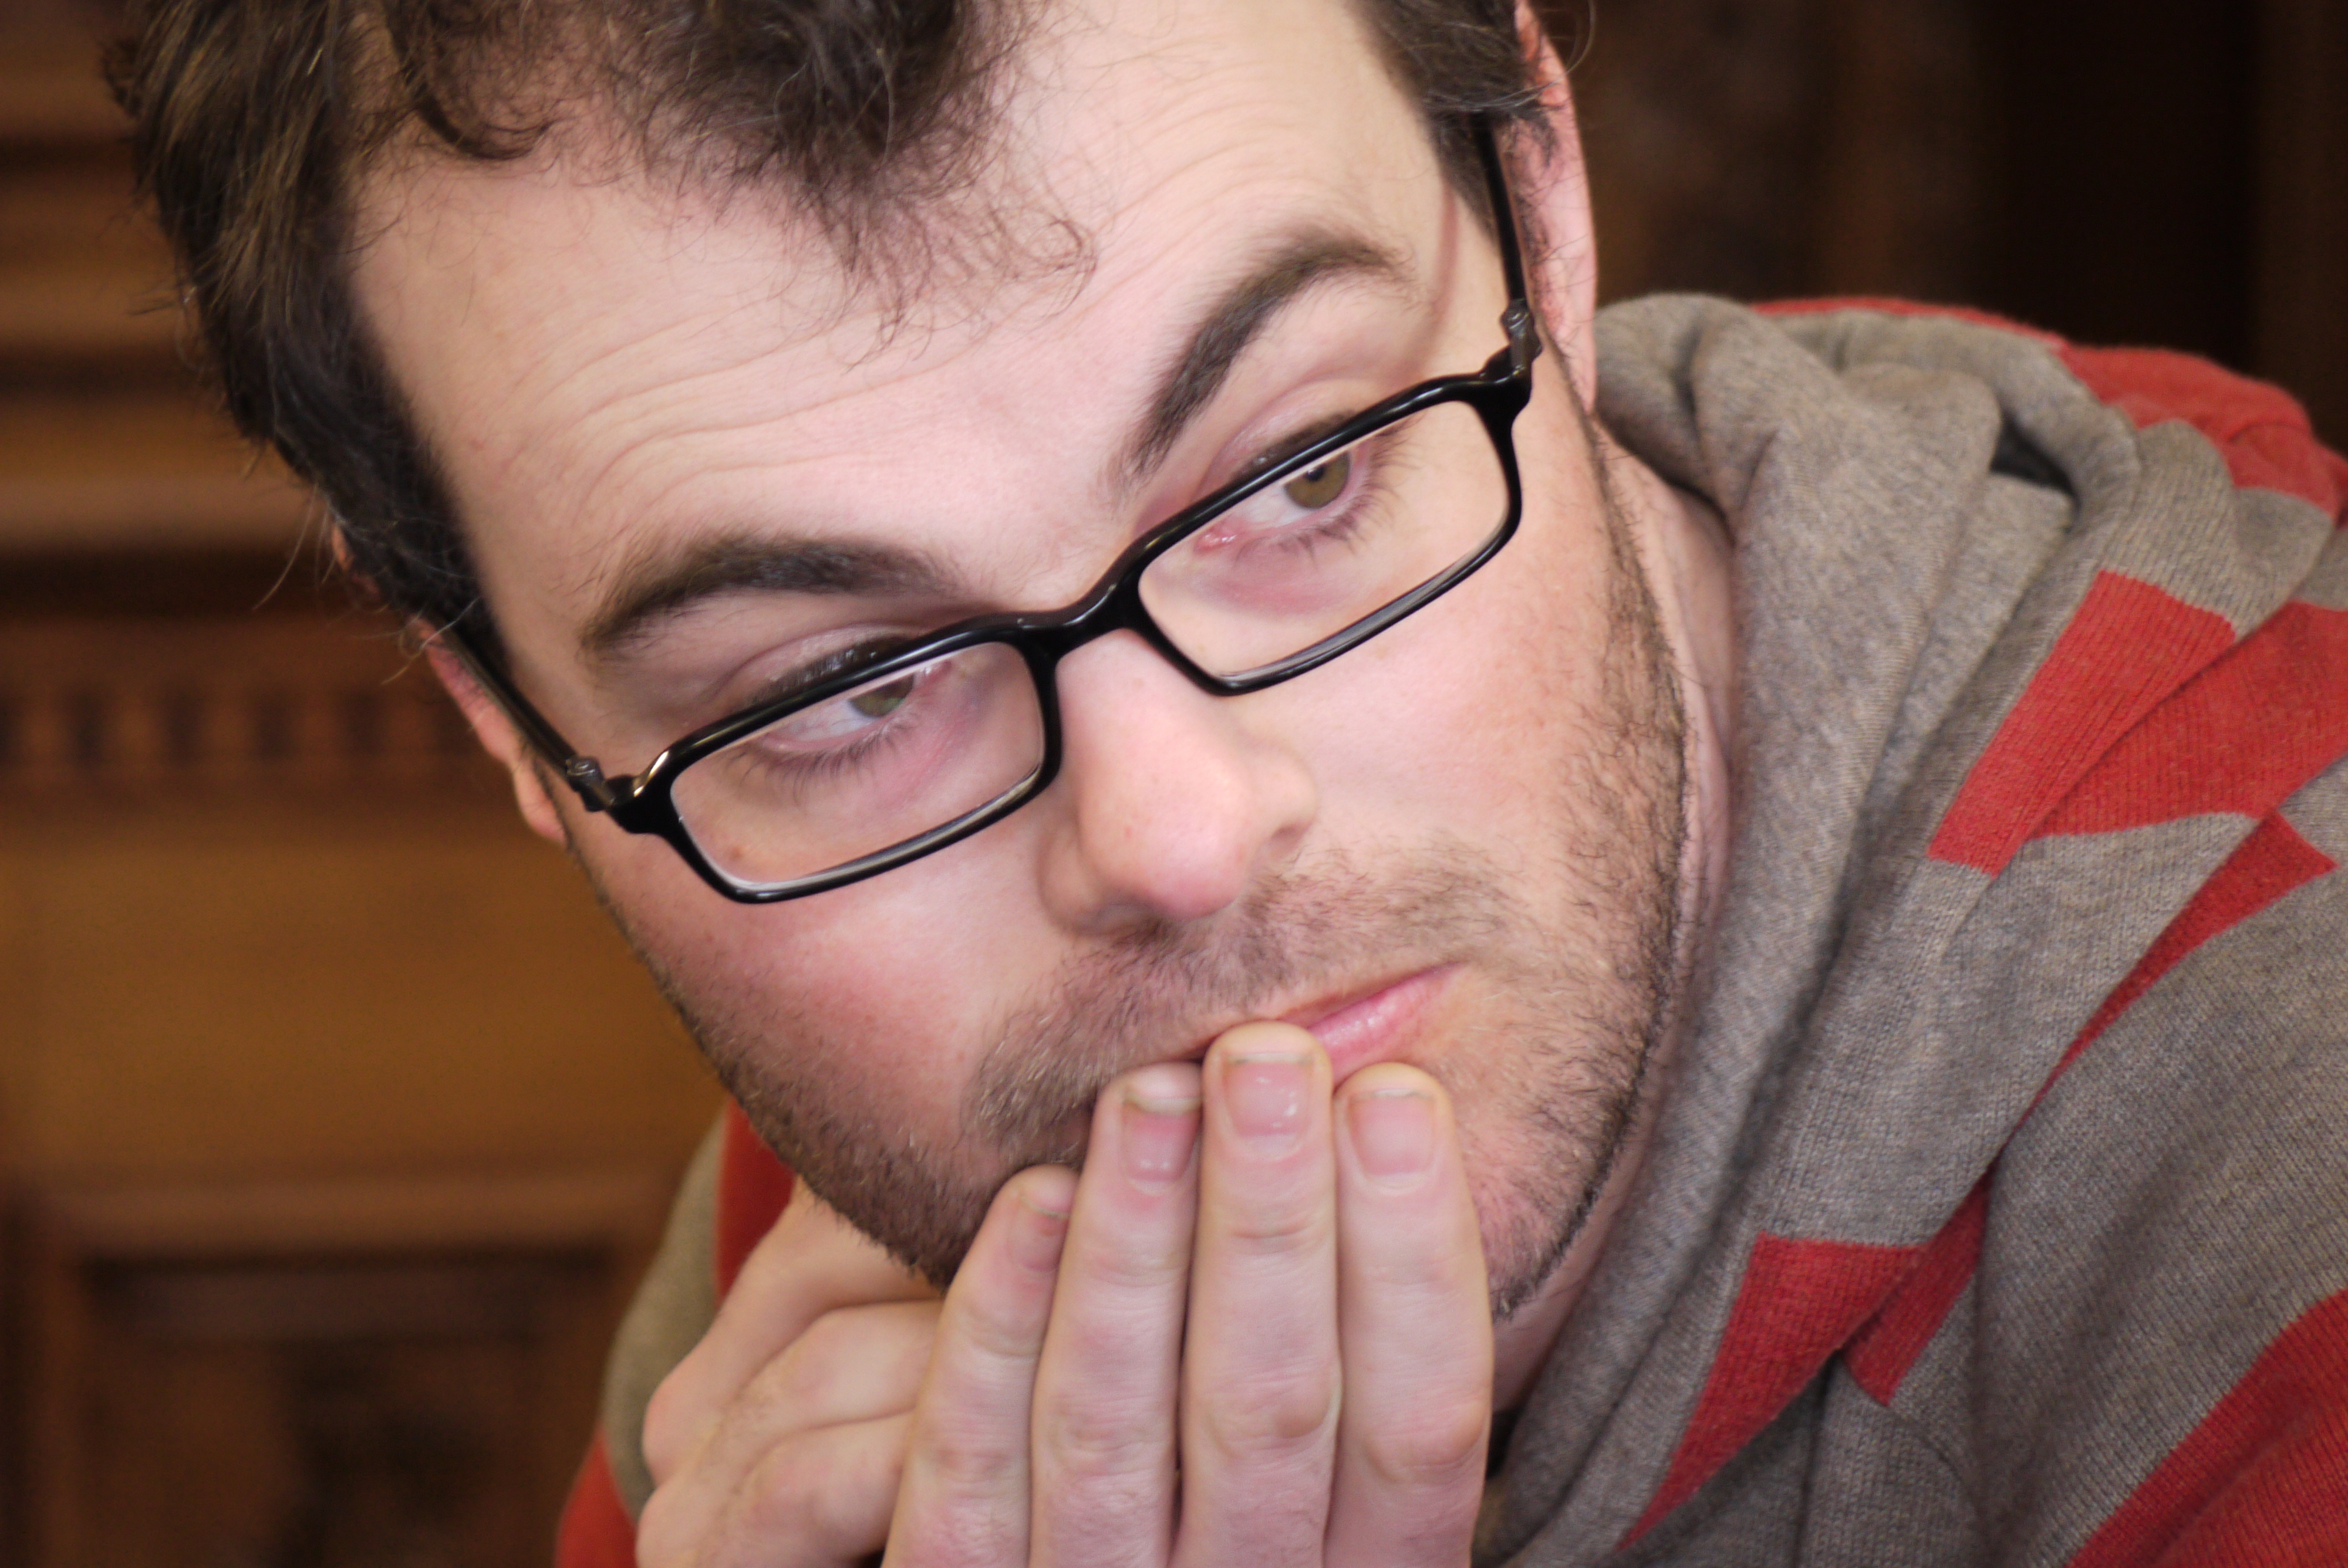
\includegraphics[trim=800px 10px 1200px 200px, clip,width=#1]{../../../photos/group/2013_03_28_112411.JPG}}
\global\long\def\teoPicture#1{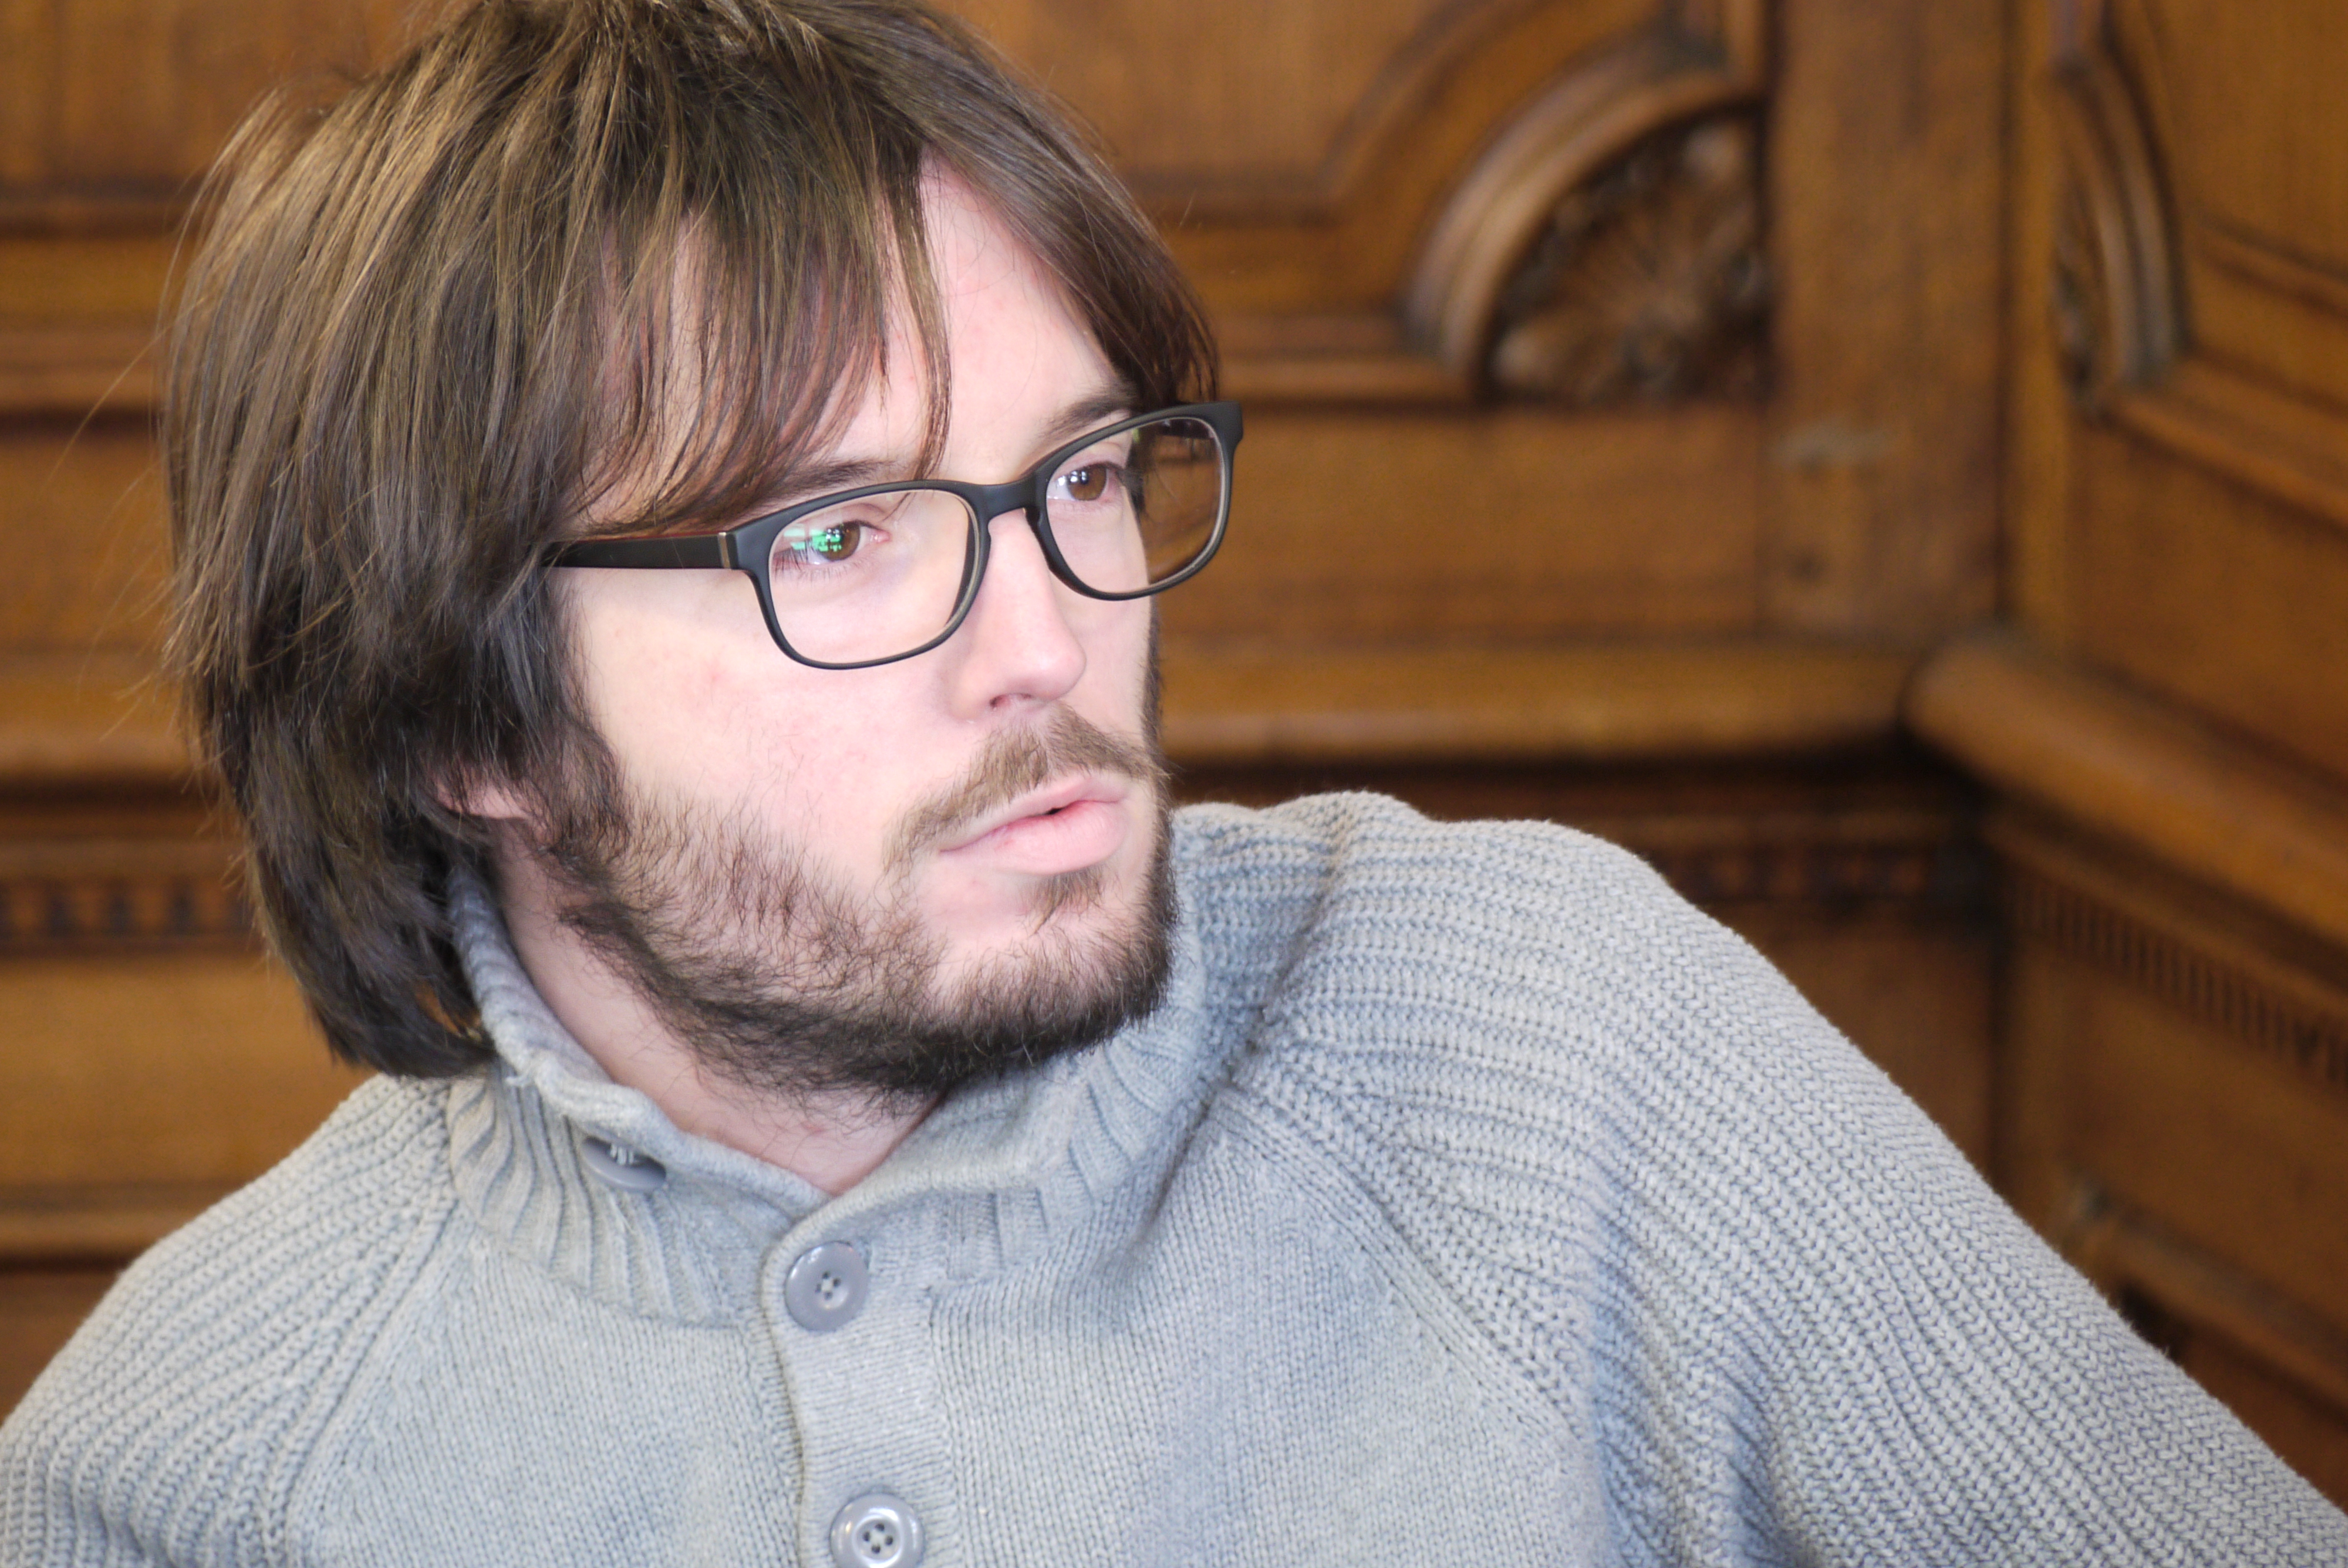
\includegraphics[trim=300px 700px 1900px 200px, clip,width=#1]{../../../photos/group/2013_03_28_114601.JPG}}
\global\long\def\alanUnsurePicture#1{\includegraphics[trim=1700px 350px 700px 350px, clip,width=#1]{../../../photos/group/2013_03_28_114919.JPG}}
\global\long\def\gpssLogo#1{\includegraphics[width=#1]{../../../gp/tex/diagrams/logo}}

\global\long\def\zhenwenPicture#1{\includegraphics[width=#1]{../../../photos/group/zhenwen.jpg}}
\global\long\def\maxPicture#1{\includegraphics[trim=40px 33px 40px 0px, clip, width=#1]{../../../photos/group/max.jpg}}
\global\long\def\javierPicture#1{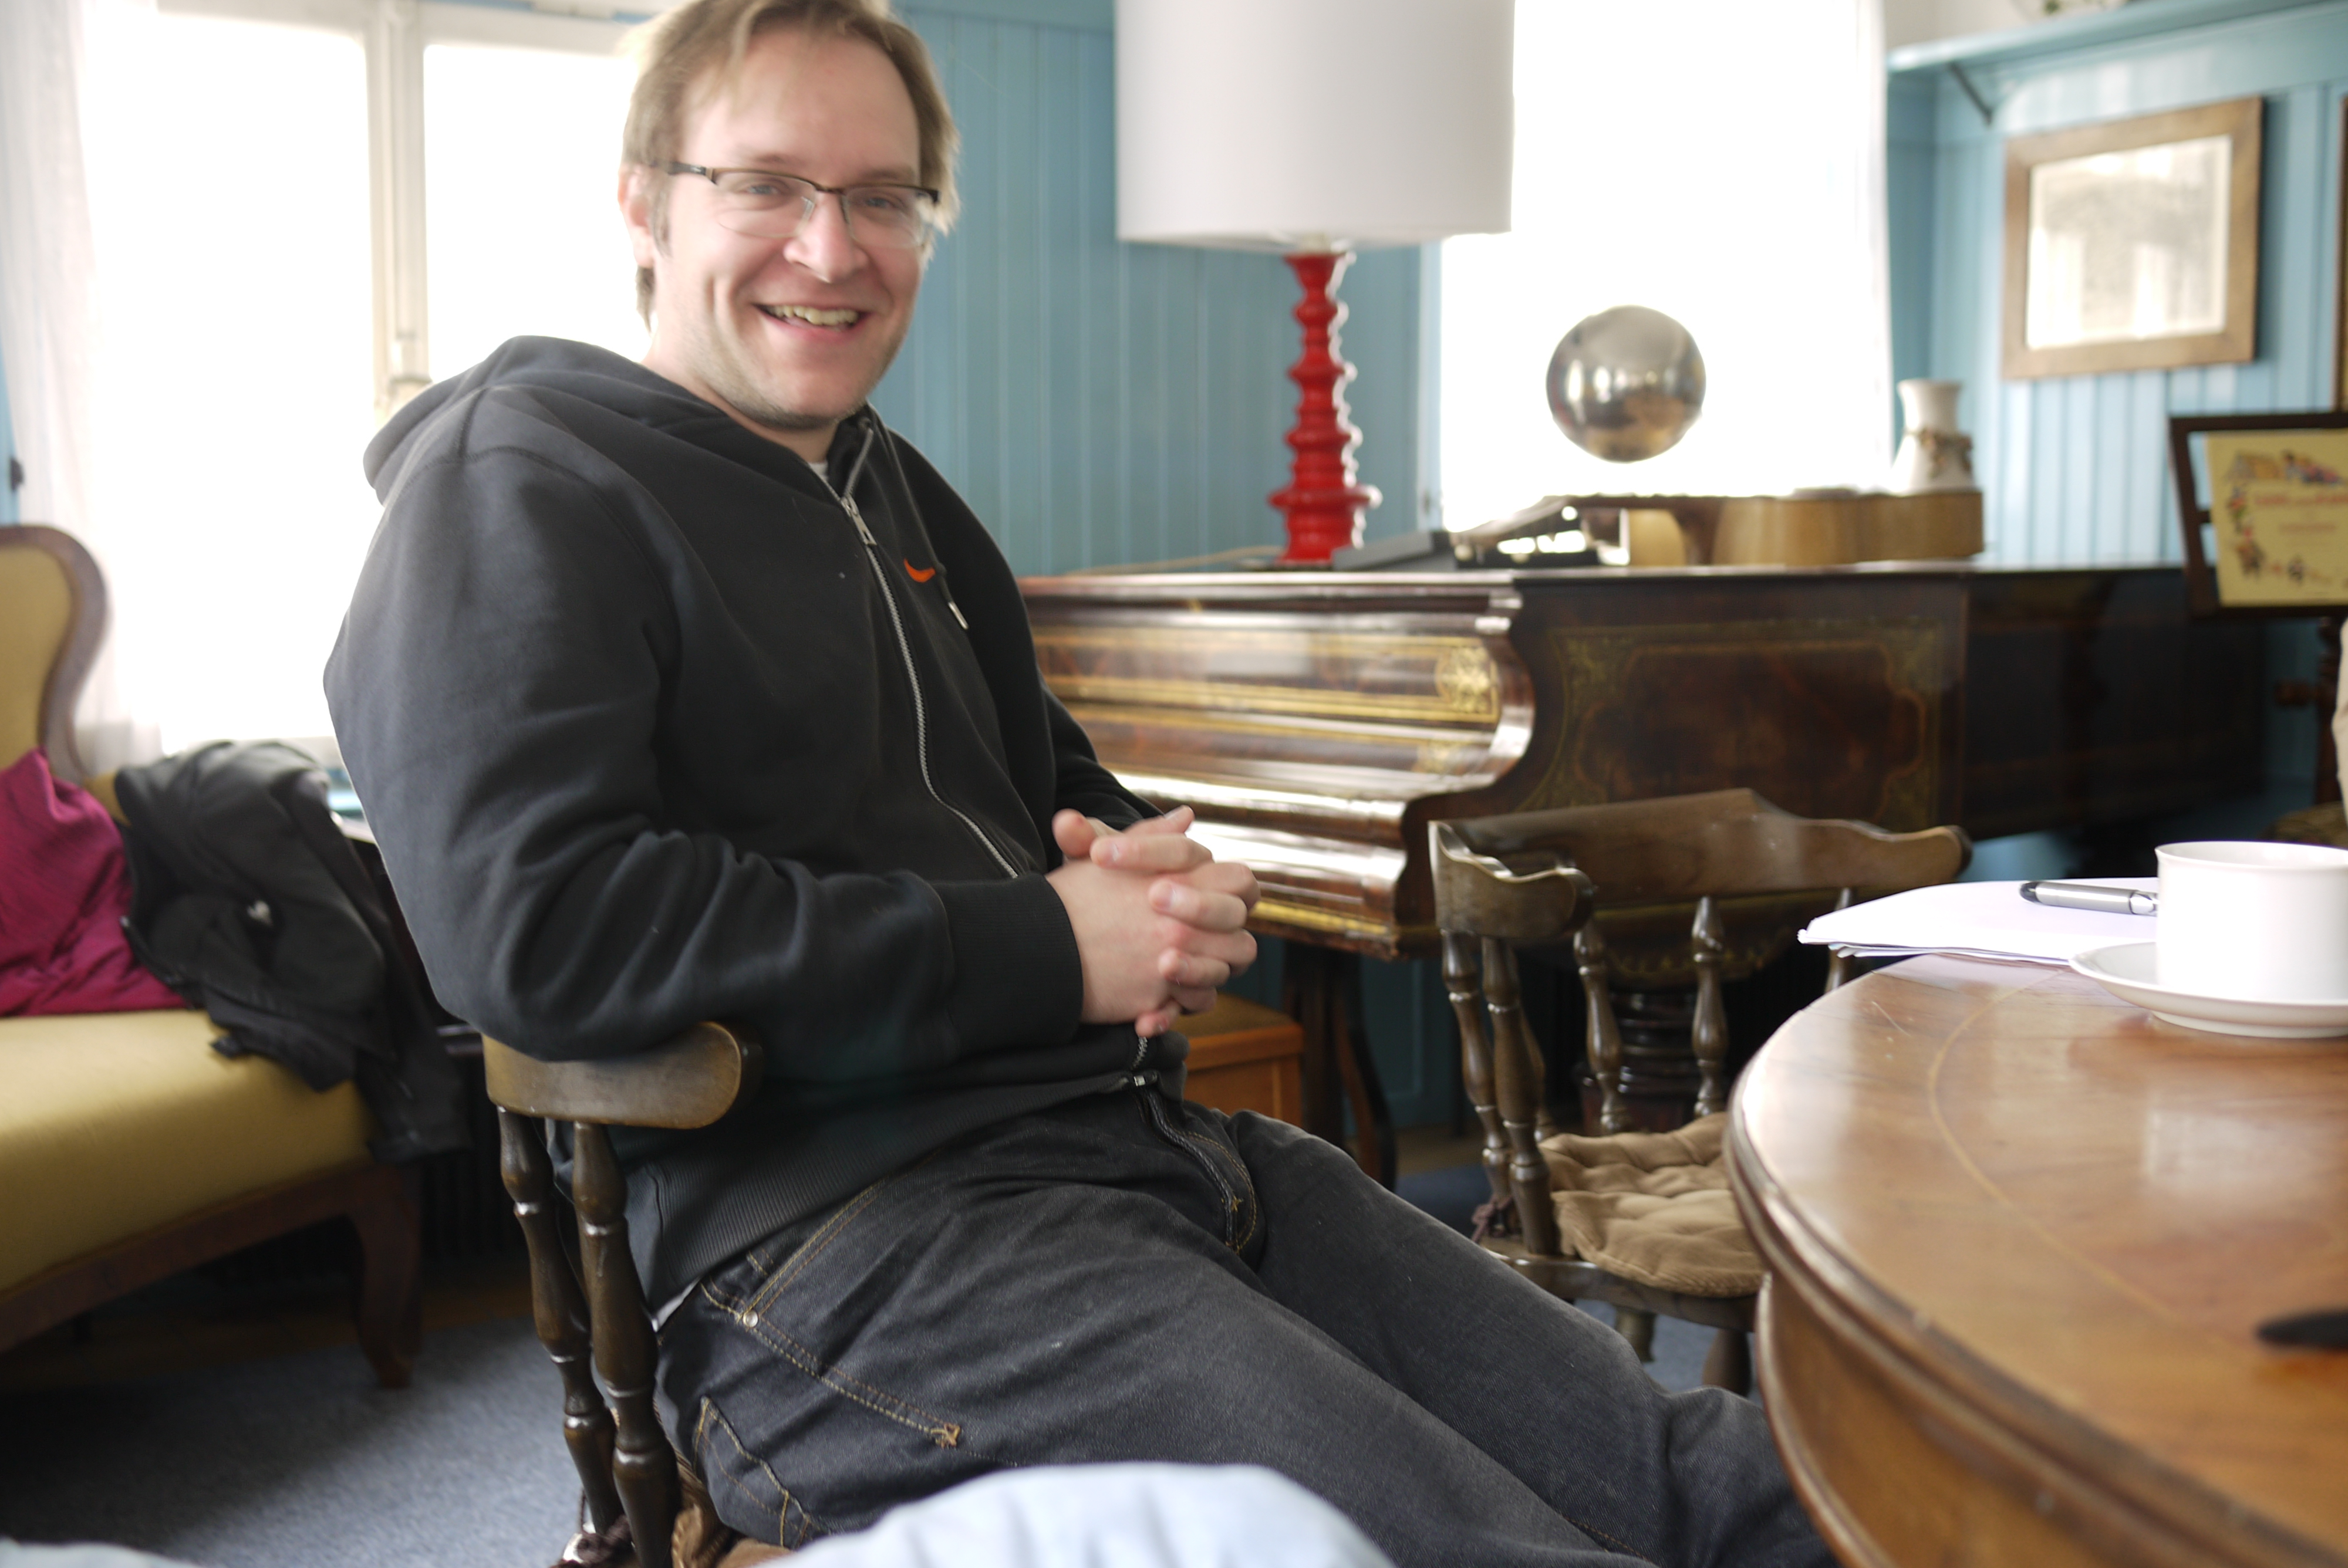
\includegraphics[trim=1026px 1909px 2333px 0px, clip,width=#1]{../../../photos/group/javier.jpg}}
\global\long\def\mikePicture#1{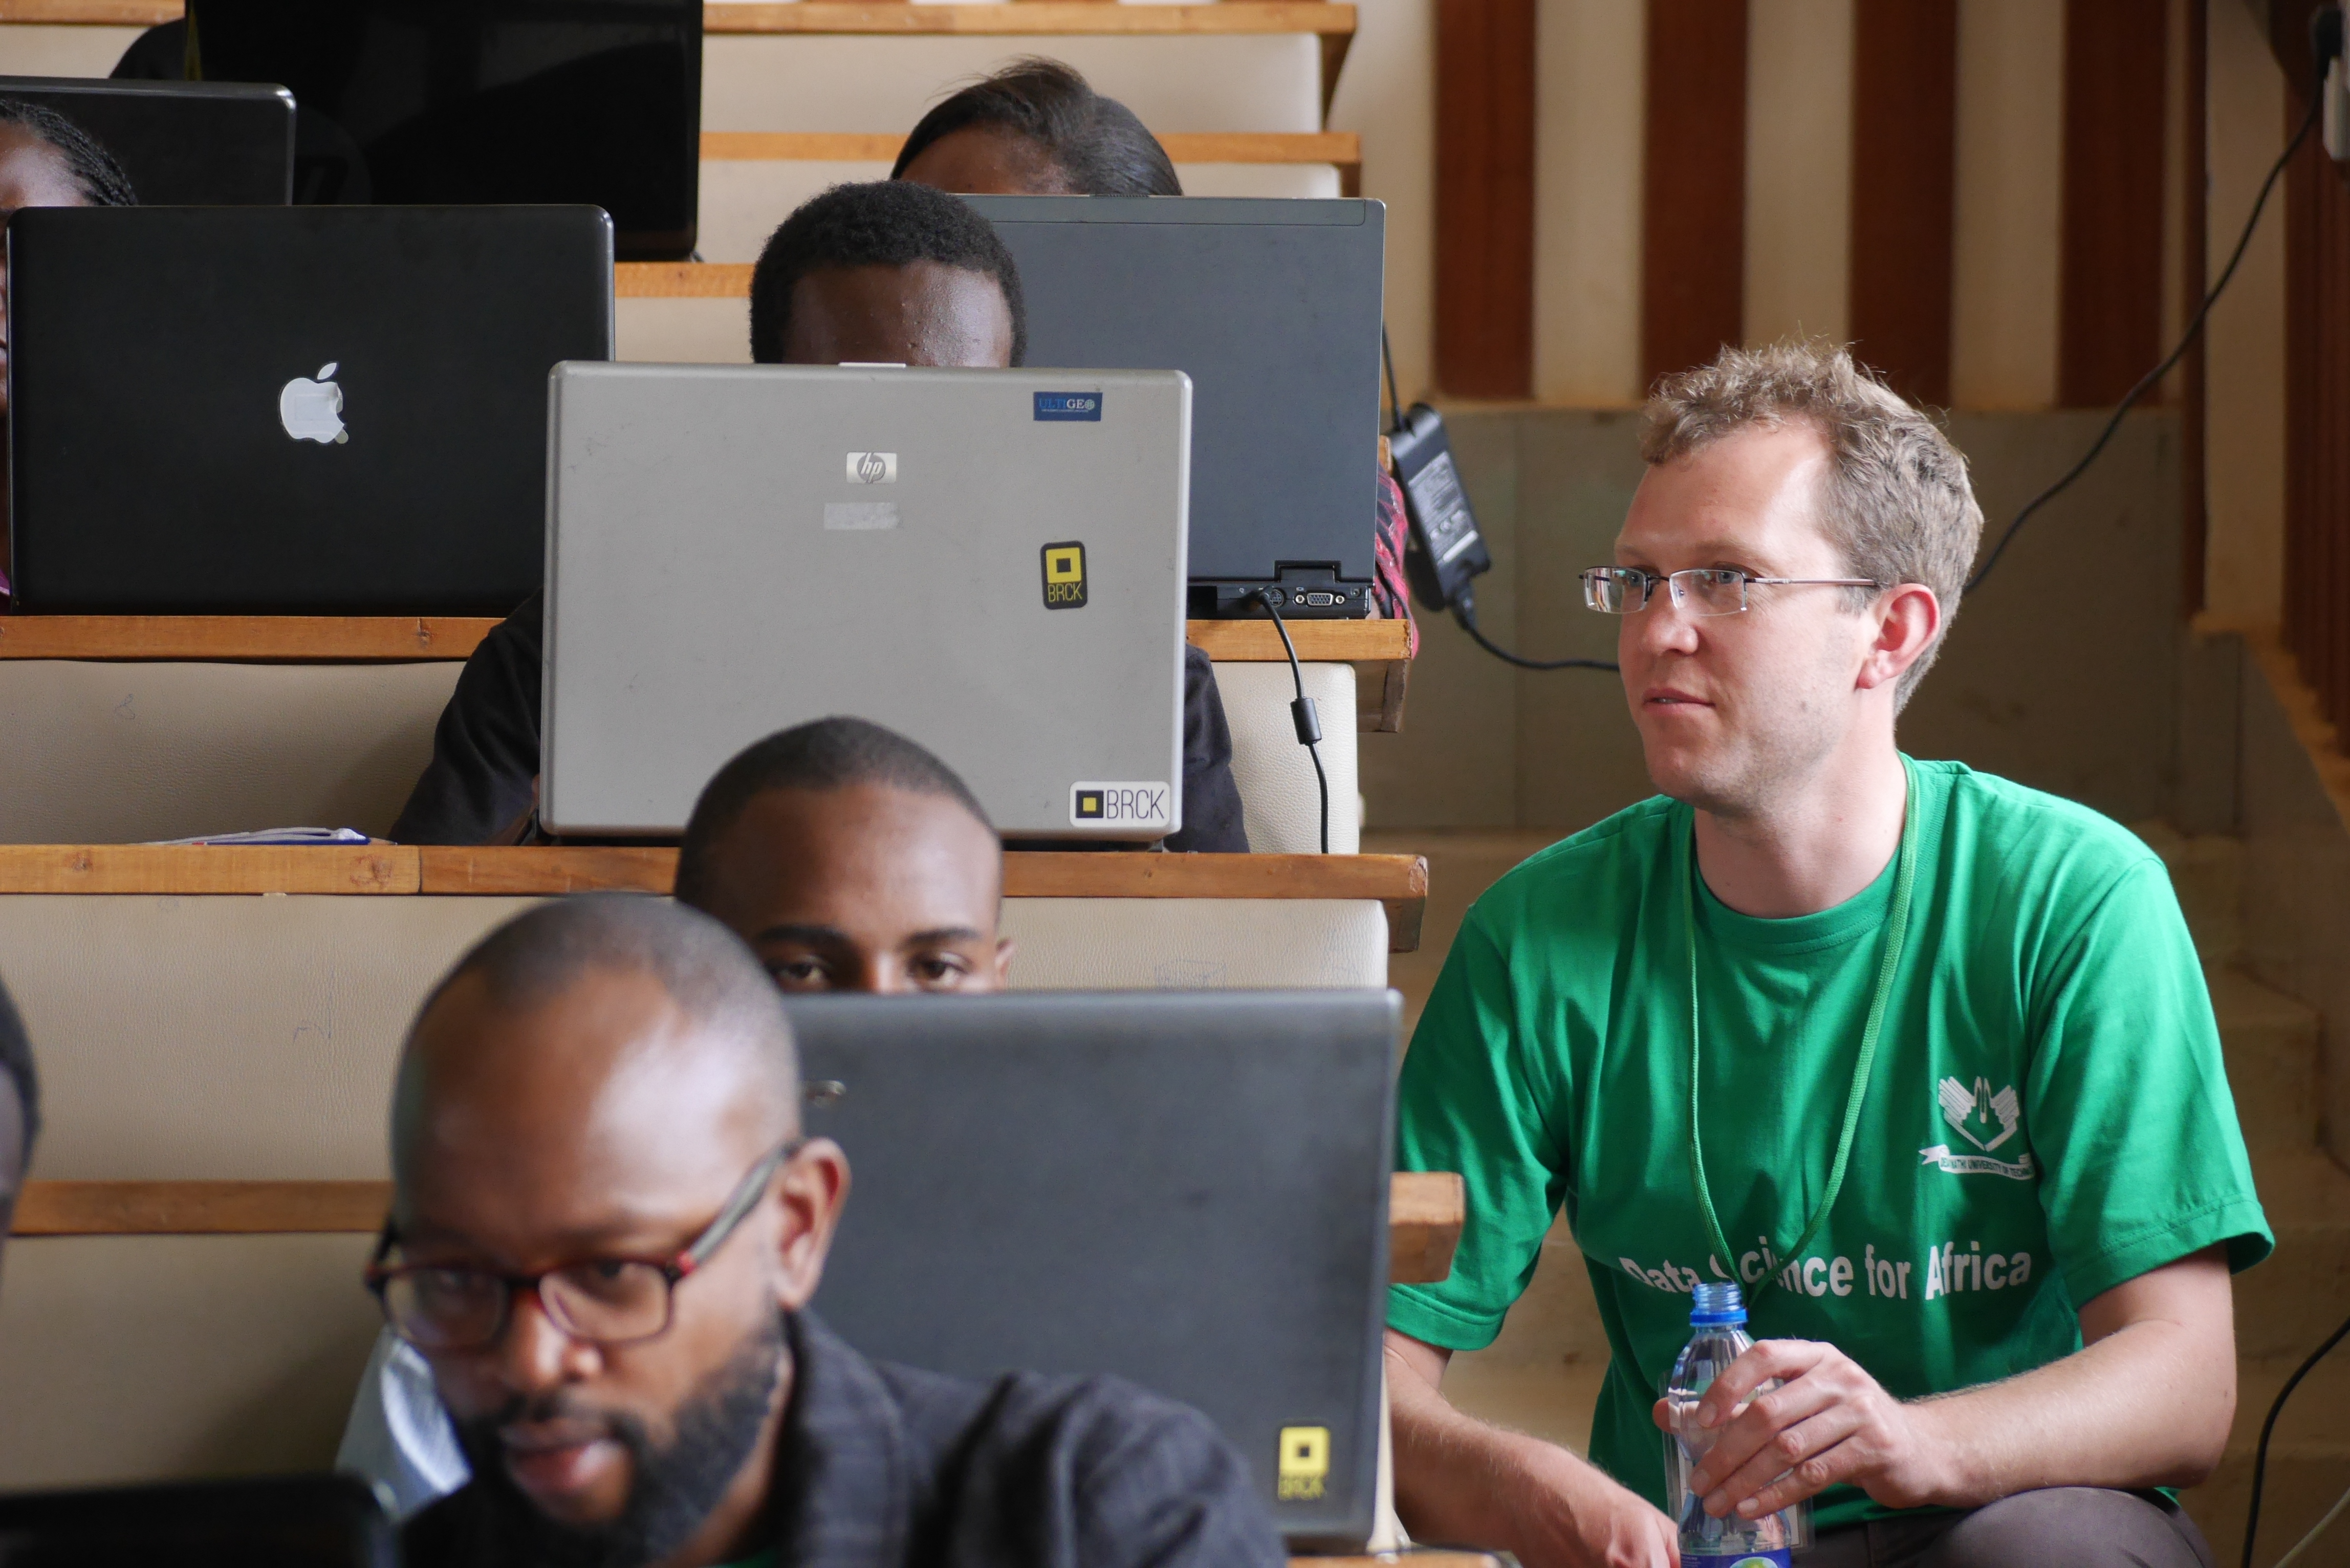
\includegraphics[trim=0px 100px 0px 648px, clip, width=#1]{../../../photos/group/2015_06_15_122941.JPG}}
\global\long\def\michalisPicture#1{\includegraphics[width=#1, trim=641px 1241px 200px 20px, clip]{../../../photos/group/michalis.jpg}}




\begin{document}
  \def\layersep{1.5cm}
  \def\nodesep{1cm}
  \pgfdeclarelayer{background}
  \pgfdeclarelayer{foreground}
  \pgfsetlayers{background,main,foreground}
  
  \begin{tikzpicture}[node distance=\layersep]
      \tikzstyle{annot} = [text width=4em, text centered]    % Draw the input layer nodes
      \begin{pgfonlayer}{foreground}


      \foreach \name / \x in {1,...,1}
      \path[xshift=\nodesep*4.5]
        node[obs] (Y-\name) at (\x*\nodesep, \layersep*0) {$\dataScalar_\x$};

        % Draw the hidden layer nodes
      \foreach \name / \x in {1,...,4}
        \path[xshift=\nodesep*3]
          node[latent] (H1-\name) at (\x*\nodesep, \layersep*1) {$\hiddenScalar^{1}_\x$};

        % Draw intermediate
      \foreach \name / \x in {1,...,2}
        \path[xshift=\nodesep*4]
          node[const] (I1-\name) at (\x*\nodesep, \layersep*1.5) {};

        % Draw the hidden layer nodes
      \foreach \name / \x in {1,...,6}
        \path[xshift=\nodesep*2]
          node[latent] (H2-\name) at (\x*\nodesep, \layersep*2) {$\hiddenScalar^{2}_\x$};


        % Draw intermediate
      \foreach \name / \x in {1,...,4}
        \path[xshift=\nodesep*3]
          node[const] (I2-\name) at (\x*\nodesep, \layersep*2.5) {};

        % Draw the hidden layer nodes
      \foreach \name / \x in {1,...,8}
        \path[xshift=\nodesep]
          node[latent] (H3-\name) at (\x*\nodesep, \layersep*3) {$\hiddenScalar^{3}_\x$};


        % Draw intermediate
      \foreach \name / \x in {1,...,4}
        \path[xshift=\nodesep*3]
          node[const] (I3-\name) at (\x*\nodesep, \layersep*3.5) {};
      

        % Draw the input layer nodes
      \foreach \name / \x in {1,...,6}
        \path[xshift=\nodesep*2]
          node[obs] (X-\name) at (\x*\nodesep, \layersep*4) {$\inputScalar_\x$};


      \end{pgfonlayer}

      \begin{pgfonlayer}{background}
      % Connect every node in the latent layer with every node in the
      % data layer.
      \foreach \source in {1,...,4}
        \foreach \dest in {1,...,1}
          \draw[->] (H1-\source) -- (Y-\dest);

      \foreach \source in {1,...,2}
        \foreach \dest in {1,...,4}
          \draw[->] (I1-\source) -- (H1-\dest);

      \foreach \source in {1,...,6}
        \foreach \dest in {1,...,2}
          \draw[->] (H2-\source) -- (I1-\dest);

      \foreach \source in {1,...,4}
        \foreach \dest in {1,...,6}
          \draw[->] (I2-\source) -- (H2-\dest);

      \foreach \source in {1,...,8}
        \foreach \dest in {1,...,4}
          \draw[->] (H3-\source) -- (I2-\dest);

      \foreach \source in {1,...,4}
        \foreach \dest in {1,...,8}
          \draw[->] (I3-\source) -- (H3-\dest);

      \foreach \source in {1,...,6}
        \foreach \dest in {1,...,4}
          \draw[->] (X-\source) -- (I3-\dest);

      \end{pgfonlayer}

      % Annotate the layers
      \node[annot,right of=X-6, node distance=2cm, text width=3cm] (ls) {given $\inputVector$};
      \node[annot,right of=I3-4, node distance=2cm, text width=3cm] (ls) {$\latentVector_{1} = \eigenvectwoMatrix^\top_1 \inputVector$};
      \node[annot,right of=H3-8, node distance=2cm, text width=3cm] (ls) {$\hiddenVector_{1} = \mathbf{g}\left(\eigenvectorMatrix_1 \latentVector_{1}\right)$};
      \node[annot,right of=I2-4, node distance=2cm, text width=3cm] (ls) {$\latentVector_{2} = \eigenvectwoMatrix^\top_2 \hiddenVector_{3}$};
      \node[annot,right of=H2-6, node distance=2cm, text width=3cm] (ls) {$\hiddenVector_{2} = \mathbf{g}\left(\eigenvectorMatrix_2 \latentVector_{2}\right)$};
      \node[annot,right of=I1-2, node distance=2cm, text width=3cm] (ls) {$\latentVector_{3} = \eigenvectwoMatrix^\top_1 \hiddenVector_{2}$};
      \node[annot,right of=H1-4, node distance=2cm, text width=3cm] (ls) {$\hiddenVector_{3} = \mathbf{g}\left(\eigenvectorMatrix_3 \latentVector_{3}\right)$};
      \node[annot,right of=Y-1, node distance=2cm, text width=3cm] (ds) {$\dataVector = \weightVector_4^\top \hiddenVector_{3}
$};
  \end{tikzpicture}
\end{document}
